\documentclass[a4paper,10pt]{report}

\usepackage{graphicx}
\usepackage{hyperref}
\usepackage{amsmath}
\usepackage{amssymb}
\usepackage{xspace}
\pagestyle{headings}
%\usepackage[total={6.5in,10in}, top=1.2in, left=.8in, includefoot]{geometry}
\usepackage[left=2cm, right=2cm, top=2.5cm, bottom=2cm]{geometry}
\usepackage{float}
\restylefloat{table}
\usepackage{listings}
\usepackage{color}
\definecolor{gray}{rgb}{0.4,0.4,0.4}
\definecolor{darkblue}{rgb}{0.0,0.0,0.58}
\definecolor{attributeColor}{rgb}{0.96,0.517,0.29}
\definecolor{darkgreen}{rgb}{0,.392,0}
\definecolor{stringColor}{rgb}{0.6,0.2,0}
\definecolor{lightgray}{rgb}{.7,.7,.7}
\newsavebox\lstbox
\usepackage{array,multirow}
\usepackage{longtable}
\LTcapwidth=\textwidth
\usepackage{cleveref}
\usepackage{bbding}
\crefname{section}{�}{��}
\Crefname{section}{�}{��}
\usepackage[utf8]{inputenc}
\usepackage{tablefootnote}
\usepackage{algorithmic}
\usepackage[modulo, pagewise]{lineno}
\nolinenumbers
\usepackage{fancyhdr}
\pagestyle{fancy}
\fancyhead[RO]{Continuous Observation Models}
\fancyhead[RE]{\itshape\nouppercase{\leftmark}}
\usepackage{booktabs}
%\fancyfoot[CE,CO]{\leftmark}
%\fancyfoot[LE,RO]{\thepage}
%\pagestyle{fancy}
%\fancyhf{}
\usepackage{array,arydshln}
\usepackage{wrapfig}

\setlength\dashlinedash{0.4pt}
\setlength\dashlinegap{1pt}
\setlength\arrayrulewidth{0.5pt}

\newcommand{\myStartLine}{\par
  \kern8pt % space above the rules
  \hrule height 0.5pt
  \kern3pt % space below the rules
}
\newcommand{\myEndLine}{\par
  \kern3pt % space above the rules
  \hrule height 1.5pt
  \kern12pt % space below the rules
}

\lstset{
  basicstyle=\ttfamily,
  columns=fullflexible,
  showstringspaces=false,
  commentstyle=\color{gray}\upshape
%  numbers=left,
%  stepnumber=5
}

\newcommand{\HRule}{\rule{\linewidth}{0.5mm}}

\lstdefinelanguage{XML}
{
  basicstyle=\ttfamily\footnotesize,
  morestring=[b]",
  morestring=[s]{>}{<},
  moredelim=[is][\bfseries\color{red}]{[*}{*]},
  moredelim=[s][\bfseries\color{darkblue}]{<}{\ },
  moredelim=[s][\bfseries\color{darkblue}]{</}{>},
  moredelim=[l][\bfseries\color{darkblue}]{/>},
  moredelim=[l][\bfseries\color{darkblue}]{>},
  morecomment=[s]{<?}{?>},
  morecomment=[s]{<![CDATA[}{]]>},
  moredelim=[s][\bfseries\color{darkgreen}]{<!--}{-->},
  commentstyle=\color{darkgreen},
  stringstyle=\color{stringColor},
  identifierstyle=\color{red},
  keywordstyle=\color{attributeColor},
  morekeywords={oid,columnId,columnIdRef,symbId,symbolType,op,columnNum,columnType,
  valueType,inputTarget,blkId,blkIdRef,symbIdRef,xmlns,version,type,VariableMapping,
  IndividualMapping,schemaLocation,xs,xsi,NONMEMdataSet,matrixType,opType,order,
  math,ct,ds,mdef,mstep,mml,un,name,definition,writtenVersion,id,inputType,oidRef,catId,
  length,default,vectorIndex,diagDefault,offDiagDefault,row,column,numbRows,numbCols,
  dataSymbol,modelSymbol,ordered,compartmentNo,compNo,ordered,linkFunction,varId,
  censoringType,dataSymbol,modelSymbol,MarkovOrder,deviationMatrixType,implementedBy,
  argument,admNumber,transformId,transformIdRef,metadataFile,fixed,toolName,dataCode,
  missingDataType} % list your attributes here
}

\lstdefinelanguage{MLX} 
{
  basicstyle=\ttfamily\footnotesize,
  morestring=[b]",
  morestring=[s]{>}{<},
  moredelim=[s][\bfseries\color{darkblue}]{<}{\ },
  moredelim=[s][\bfseries\color{darkblue}]{</}{>},
  moredelim=[l][\bfseries\color{darkblue}]{/>},
  moredelim=[l][\bfseries\color{darkblue}]{>},
  morecomment=[s]{<?}{?>},
  morecomment=[s]{<!--}{-->},
  morecomment=[s]{<![CDATA[}{]]>},
  commentstyle=\color{darkgreen},
  stringstyle=\color{stringColor},
  identifierstyle=\color{black},
  keywordstyle=\color{attributeColor},
  morekeywords={dads} % list your attributes here
}

\lstdefinelanguage{NM}
{
  basicstyle=\sffamily\small,
  morestring=[b]",
  morestring=[s]{>}{<},
  moredelim=[is][\bfseries\color{red}]{[*}{*]},
  moredelim=[s][\bfseries\color{darkblue}]{<}{\ },
  moredelim=[s][\bfseries\color{darkblue}]{</}{>},
  moredelim=[l][\bfseries\color{darkblue}]{/>},
  moredelim=[l][\bfseries\color{darkblue}]{>},
  morecomment=[s]{<?}{?>},
  morecomment=[s]{<!--}{-->},
  morecomment=[s]{<![CDATA[}{]]>},
  commentstyle=\color{darkgreen},
  stringstyle=\color{stringColor},
  identifierstyle=\color{black},
  keywordstyle=\color{attributeColor},
  morekeywords={kjkj} % list your attributes here
}


\lstdefinelanguage{Elements}
{
  basicstyle=\sffamily\footnotesize,
  morestring=[b]",
  morestring=[s]{>}{<},
  moredelim=[s][\bfseries\color{darkblue}]{<}{\ },
  moredelim=[s][\bfseries\color{darkblue}]{</}{>},
  moredelim=[l][\bfseries\color{darkblue}]{/>},
  moredelim=[l][\bfseries\color{darkblue}]{>},
  morecomment=[s]{<?}{?>},
  morecomment=[s]{<!--}{-->},
  morecomment=[s]{<![CDATA[}{]]>},
  commentstyle=\color{darkgreen},
  stringstyle=\color{stringColor},
  identifierstyle=\color{black},
  keywordstyle=\color{attributeColor},
  morekeywords={kjkj} % list your attributes here
}

\newcommand{\cellml}{CellML\xspace}
\newcommand{\sbml}{SBML\xspace}
\newcommand{\sedml}{SED-ML\xspace}
\newcommand{\mathml}{MathML\xspace}
\newcommand{\uncertml}{UncertML\xspace}
\newcommand{\pml}{PharmML\xspace}
\newcommand{\pharmml}{PharmML\xspace}
\newcommand{\xelem}[1]{\texttt{<#1>}\index{XML Element!\texttt{<#1>}}}
\newcommand{\xatt}[1]{\texttt{#1}\index{XML Attribute!\texttt{#1}}}


\begin{document}


\begin{titlepage}
\begin{center}

% Upper part of the page. The '~' is needed because \\
% only works if a paragraph has started.

\includegraphics[width=0.35\textwidth]{./logo/ddmore_logo}~\\[1cm]

%\textsc{\LARGE }\\[1.5cm]
%
\textsc{\Large Technical Report}\\[0.5cm]

% Title
\HRule \\[0.4cm]
{ \huge \bfseries Continuous Observation Models \\[0.4cm] }
{ \large \bfseries With NMTRAN/MLXTRAN code \\[0.4cm] }

\HRule \\[1.5cm]


% Authors
\begin{minipage}{0.9\textwidth}
\begin{flushleft} \large
Maciej J \textsc{Swat}$^1$, Roberto \textsc{Bizzotto}$^2$, Marc \textsc{Lavielle}$^3$ \\
\end{flushleft}
\end{minipage}


\bigskip
\begin{minipage}{0.9\textwidth}
\begin{flushleft} \large
$^1$\emph{EMBL - European Bioinformatics Institute, Cambridge, UK} \\ 
$^2$\emph{National Research Council, Institute of Neuroscience, Padova, Italy} \\
$^3$\emph{Inria Saclay, France}
\end{flushleft}
\end{minipage}


\bigskip
\vfill

\textcolor{red}{WORKING DRAFT VERSION}

\vfill

% Bottom of the page
{\large \today \\}

\end{center}
\end{titlepage} 

\linenumbers
\tableofcontents

%%%%%%%%%%%%%%%%%%%%%%%%%%%%%%%%%%%%%%%%%%%%%%%%%%%%%%%%%%%%%%%%
%%%%%%%%%%%%%%%%%%%%%%%%%%%%%%%%%%%%%%%%%%%%%%%%%%%%%%%%%%%%%%%%
%%%%%%%%%%%%%%%%%%%%%%%%%%%%%%%%%%%%%%%%%%%%%%%%%%%%%%%%%%%%%%%%


%\appendix
%%%%%%%%%%%%%%%%%%%%%%%%%%%%%%%%%%%%%%%%%%%%%%%%%%%%%%%%%%%%%%%%
%%%%%%%%%%%%%%%%%%%%%%%%%%%%%%%%%%%%%%%%%%%%%%%%%%%%%%%%%%%%%%%%%%%%%%%%
\chapter{Introduction}
\label{cht:intro}

The purpose of this document is to discuss observation models
used in nonlinear mixed effects (NLME) models for continuous data 
and supported in PharmML, \cite{Pharmml_06}. It starts with a 
general classification of observation models and discusses aspects of the 
variability structure of residual error models.
A short overview of the most common models follows which are then 
described in detail in chapter \ref{sec:typicalResModel}. Chapter \ref{ch:otherModels} 
discusses then a number of non-standard models, among others from the 
\cite{Keizer:2013aa}.


\section{Classification of observation models} % \textcolor{red}{changes}
\label{sec:modelClassific}

The observation models can be divided into three groups:
\begin{itemize}
\item 
\textbf{Structured} models (\textbf{S-type})
\begin{itemize}
\item 
\textbf{General model} -- residual error, $\epsilon_{ij}$, with a symmetric distribution with mean 0
\begin{itemize}
 \item
for \textbf{transform-both-sides} data
\begin{eqnarray}
 \underbrace{ u(y_{ij})}_{\text{\parbox{2cm}{\centering Transformed \\[-4pt] experimental \\[-4pt]  data}}} =
 \underbrace{ u\big(f(x_{ij}, \psi_{i})\big)}_{\text{\parbox{2.5cm}{\centering Transformed \\[-4pt]  model \\[-4pt]  prediction}}} +
 \underbrace{ g(x_{ij}, \psi_{i}, \xi_i) \; \epsilon_{ij}}_{\text{\parbox{3cm}{\centering Residual \\[-4pt] error}}}
 \end{eqnarray}
\item
for \textbf{untransformed} data  -- special case of the previous with $h \equiv identity$ 
\begin{eqnarray}
 \underbrace{ y_{ij}}_{\text{\parbox{2cm}{\centering Experimental \\[-4pt]  data}}} =
 \underbrace{ f(x_{ij}, \psi_{i})}_{\text{\parbox{2.5cm}{\centering Model \\[-4pt]  prediction}}} +
 \underbrace{ g(x_{ij}, \psi_{i}, \xi_i) \; \epsilon_{ij}}_{\text{\parbox{3cm}{\centering Residual \\[-4pt] error}}}
 \nonumber
 \end{eqnarray}
\end{itemize}
\item
\textbf{Gaussian model} --  special case of eq. (1.1) with $\epsilon_{ij} \sim \mathcal{N}(0,1)$ --
$u(y_{ij})$ is normally distributed with mean $u(f(x_{ij}, \psi_{i}))$ and the 
standard deviation $g(x_{ij}, \psi_{i}, \xi_i)$. 

\end{itemize}
\item 
\textbf{Distribution} based models (\textbf{D-type})
\begin{align}
	& u(y_{ij})  \sim DistributionName(parameter1, parameter2, ...)
\end{align}
\item
\textbf{Equation} based models  (\textbf{E-type})
\begin{eqnarray}
 \underbrace{ u(y_{ij})}_{\text{\parbox{2cm}{\centering Transformed \\[-4pt] experimental \\[-4pt]  data}}} =
 \underbrace{ U\big(f(x_{ij}, \psi_{i}),\xi_i, \epsilon_{1,ij}, \epsilon_{2,ij}, \dots\big)}_{\text{\parbox{3.5cm}{\centering Transformed \\[-4pt]  model prediction \\[-4pt]  including residual errors}}}
 \end{eqnarray}
\end{itemize}
Symbol description:
\begin{itemize}
\item	
$1\le i \le N$
\item
$1\le j \le n_i$
\item
$y_{ij}$ -- $j^{th}$ observation for subject $i$
\item
$f$ -- structural model prediction
\item
$x_{ij}$ -- regression variables, e.g. time or concentration
\item
$\psi_{i}$ -- individual parameters
\item
$\epsilon_{ij}$ -- normalised residual error
\item
$g$ -- standard deviation of the residual error
\item
$\xi_i$ -- parameters of the residual model.
\end{itemize}
%Type (1) is a special case of type (2) with $u \equiv Id$, i.e. the identity transformation. 
%Then for models of type (1) and (2) with $\epsilon_{ij}$ being normal distributed with 
%mean 0 and variance 1, 

%\subsection{Note of BTS - FINISH}
%Models for the standard deviation $g(x_{ij}, \psi_{i}, \xi_i)$ discuss in previous 
%section apply also in the case of \textbf{transform-both-sides} approach.
%\paragraph{Note}
%Models listed below are the most popular ones in use but the present PharmML 
%structure allows for implementation of virtually any user-defined transformation.

%\subsection{Classification and interoperability}
%\label{sec:interopGoals}
%


\section{Variability structure}
\label{sec:variabStructure}
In most cases the variability structure is reduced to one level, that of the 
observation, and its magnitude is equal among the entire population. 
However, in general, the magnitude of the residual error can vary between 
subjects or occasions. Essay errors are another variability source, the  
so called inter-replicates variability.

\subsection{Inter-individual/occasion variability (IIV/IOV)}
\label{subsec:IIVonResidualError}
In analogy to the nested hierarchical structure for the variability of the 
individual parameters, see \cite{Pharmml_06}, the variability of residual 
error parameters inherits the same structure. This way one can capture 
the inter-individual and/or inter-occasion variability of the residual error parameters.
The IIV on the residual error parameters, i.e. the varying magnitude of 
residual error between subjects, corresponds to the so 
called 'ETA-on-EPS' approach, see Figure \ref{fig:IOV0_residualError}.

\begin{figure}[htb!]
\centering
  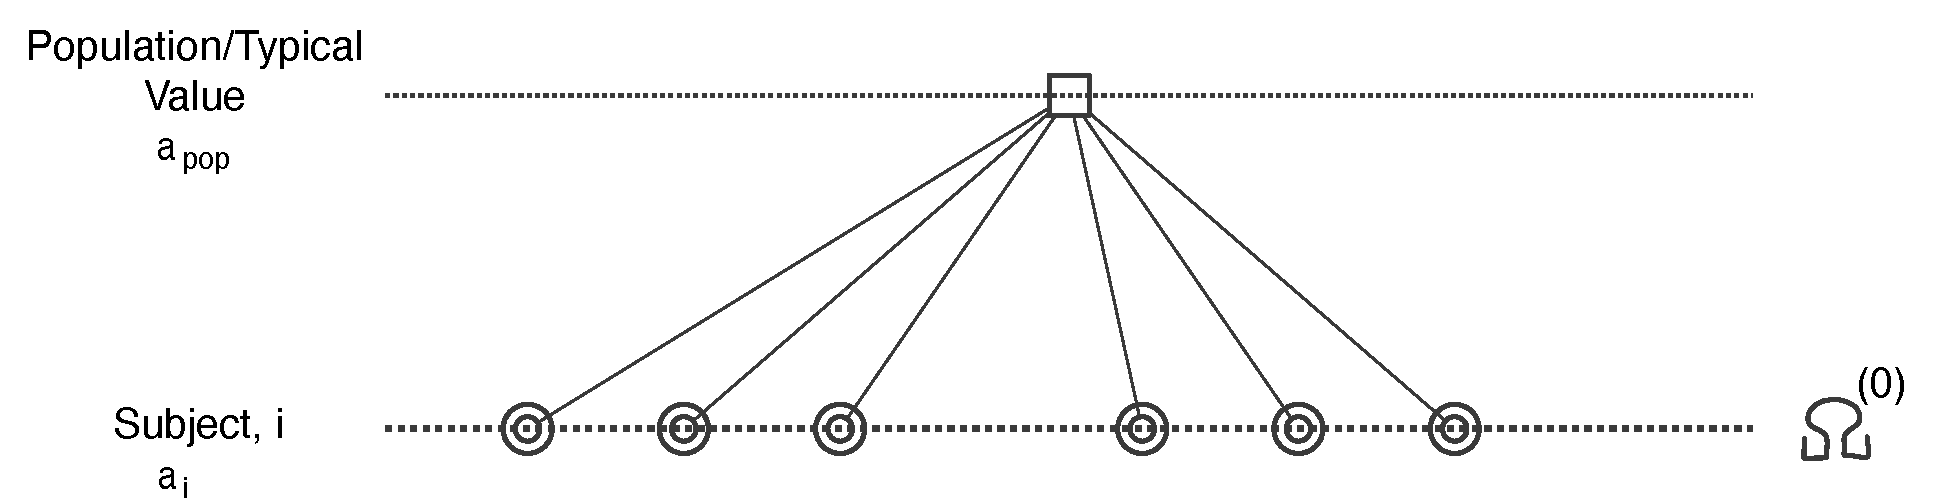
\includegraphics[width=140mm]{pics/IOV0_residualError.pdf}
 \caption{Inter-individual variability of the residual error parameter, $a$, visualised 
 as basic nested hierarchy.}
 \label{fig:IOV0_residualError}
\end{figure}

For example, if additive residual error model and log-normal distribution 
for $a$ is assumed, then the parameter model reads
\begin{eqnarray}
	&& \log(a_i) \sim \mathcal{N}(\log(a_{pop}) , \omega_a^2) \nonumber
\end{eqnarray}
and the observation model reads
\begin{eqnarray}
	&& y_{ij} \sim \mathcal{N}(f_{ij},a_i^2): \quad y_{ij} = f_{ij} + a_i \epsilon_{ij}, \quad \epsilon_{ij} \sim \mathcal{N}(0,1)	\nonumber
\end{eqnarray}
See also chapter \ref{ch:otherModels} for IIV and IOV examples with NMTRAN and MLXTRAN code.

\subsection{Inter-replicate variability (IRV)}
This variability type is analog to the inter-occasion variability for parameters,
see for example \cite{LavielleBook:2014}, and has been first considered and described in the 
literature by \cite{Karlsson:1995rm}. The replicate level in this residual error 
is described by an additional random effect and reads  
\begin{eqnarray}
	&& y_{ijk} = f_{ij} + \epsilon_{ij} + \epsilon_{ijk}, \text{ with } \epsilon_{ij} \sim \mathcal{N}(0,\Sigma^{(0)}), \epsilon_{ijk} \sim \mathcal{N}(0,\Sigma^{(1)}) 	\nonumber
\end{eqnarray}
with the $k$ index for the replicates and can therefore be visualised graphically 
in a very clear nested hierarchical structure, Figure \ref{fig:IRV_residualError}.
\begin{figure}[htb!]
\centering
  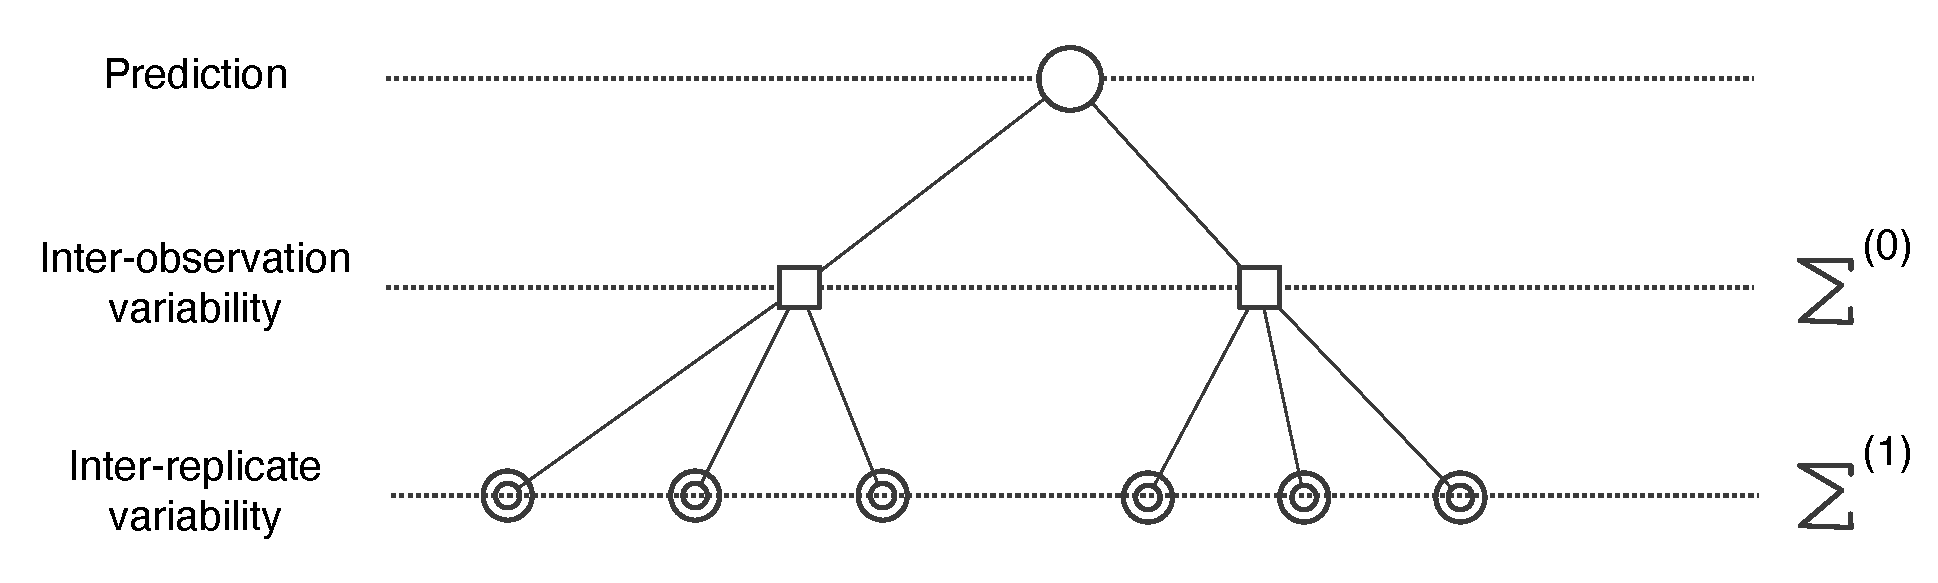
\includegraphics[width=140mm]{pics/IRV_residualError}
 \caption{Inter-replicate variability in the residual error, visualised 
 as nested hierarchy.}
 \label{fig:IRV_residualError}
\end{figure}
Each level can be fully described by a covariance matrix, $\Sigma$.

\smallskip
See also chapter \ref{ch:otherModels} for IRV examples with NMTRAN and MLXTRAN code.

\section{Selected observation model types}
In the following we list a selection of commonly used observation/residual error models, 
based mainly on \cite{NONMEM:2006aa} and \cite{LavielleBook:2014}, and described 
in detail in the next chapters:
\begin{enumerate}
\item
Constant/additive:
\begin{center} $y_{ij} = f_{ij} + a \; \epsilon_{ij}; \quad \epsilon_{ij} \sim N(0,1)$ \end{center}
\begin{center} OR $\quad y_{ij} = f_{ij} + \epsilon_{ij}; \quad \epsilon_{ij} \sim N(0,\sigma^2)$ \end{center}
\item
Constant/additive for log-transformed data, aka \emph{exponential}:
\begin{center} $\log(y_{ij}) = \log(f_{ij}) + a \epsilon_{ij}; \quad \epsilon_{ij} \sim N(0,1) \Longleftrightarrow  y_{ij} = f_{ij} \exp(a\,\epsilon_{ij})$ \end{center}
\item
Constant/additive for logit-transformed data:
\begin{center} $\displaystyle\log\Big(\frac{y_{ij}}{1-y_{ij}}\Big) = \log\Big(\frac{f_{ij}}{1-f_{ij}}\Big) + g\epsilon_{ij} \Longleftrightarrow y_{ij} = \frac{f_{ij} \exp(g\,\epsilon_{ij})}{1+f_{ij}\big(\exp(g\,\epsilon_{ij}) - 1\big)}$ \end{center}
\item
Constant/additive for extended-logit-transformed data: 
\begin{center} $\displaystyle\log\Big(\frac{y_{ij} - A}{B-y_{ij}}\Big) = \log\Big(\frac{f_{ij}-A}{B-f_{ij}}\Big) + g\,\epsilon_{ij} 
 \Longleftrightarrow y_{ij} = A + (B-A) \frac{f_{ij}-A}{f_{ij} - A + (B-f_{ij})\exp(-g\,\epsilon_{ij})} $ \end{center}
\item
Constant/additive for Box-Cox transformed data: 
\begin{center} $
\left\{ \begin{array}{lcl}  \big(y_{ij}^\lambda - 1\big)/\lambda = \big(f_{ij}^\lambda - 1\big)/\lambda + g\,\epsilon_{ij} & \mbox{for} & \lambda  \neq 0  \\
\log(y_{ij})  = \log(f_{ij}) + g\,\epsilon_{ij}  & \mbox{for} & \lambda = 0
\end{array}\right.
\Longleftrightarrow \left\{ \begin{array}{lcl}  y_{ij} = \big(f_{ij}^\lambda + \lambda g\, \epsilon_{ij} \big)^{1/ \lambda}& \mbox{for} & \lambda \neq 0  \\
y_{ij} = f_{ij} \exp(g\,\epsilon_{ij})  & \mbox{for} & \lambda  = 0
\end{array}\right.$
\end{center}
\item
Proportional or constant coefficient of variation (CCV):
\begin{center}  $y_{ij} =  f_{ij} + bf_{ij} \; \epsilon_{ij}; \quad \epsilon_{ij} \sim N(0,1)$ \end{center}
\begin{center} OR $\quad y_{ij} =  f_{ij}(1+\epsilon_{ij}); \quad \epsilon_{ij} \sim N(0,\sigma^2)$ \end{center}
\item
Combined proportional 1:
\begin{center}  $y_{ij} =  f_{ij} + (a + bf_{ij}) \; \epsilon_{ij}; \quad \epsilon_{ij} \sim N(0,1)$ \end{center}
\item
Combined proportional 2:
\begin{center}  $y_{ij} =  f_{ij} + \sqrt{a^2 + b^2f_{ij}^2} \; \epsilon_{ij}; \quad \epsilon_{ij} \sim N(0,1)$ \end{center}
\begin{center} OR $\quad y_{ij} =  f_{ij} +  a\, \epsilon_{1,ij} + b f_{ij}\, \epsilon_{2,ij}; \quad \epsilon_{1,ij} \sim N(0,1); \quad \epsilon_{2,ij} \sim N(0,1) $ \end{center}
\begin{center} OR $\quad y_{ij} =  f_{ij} (1 + \epsilon_{1,ij}) + \epsilon_{2,ij}; \quad \epsilon_{1,ij} \sim N(0,\sigma_1^2); \quad \epsilon_{2,ij} \sim N(0,\sigma_2^2)$ \end{center}
\item
Power error model: 
\begin{center}  $y_{ij} = f_{ij} + b\,f_{ij}^c \; \epsilon_{ij}; \quad \epsilon_{ij} \sim N(0,1)$ \end{center}
\begin{center}  OR $y_{ij} = f_{ij} + f_{ij}^c \; \epsilon_{ij}; \quad \epsilon_{ij} \sim N(0,\sigma^2)$\end{center}
\item
Combined power error model 1:
\begin{center}  $y_{ij} =  f_{ij} + (a + b f_{ij}^c) \; \epsilon_{ij}; \quad \epsilon_{ij} \sim N(0,1)$ \end{center}
\item
Combined power error model 2:
\begin{center}  $y_{ij} = f_{ij} + a\epsilon_{1,ij} + b f_{ij}^c \epsilon_{2,ij}; \quad \epsilon_{1,ij} \sim N(0,1); \quad \epsilon_{2,ij} \sim N(0,1)$ \end{center}
\begin{center} OR  $\quad y_{ij} = f_{ij} + \epsilon_{1,ij} + f_{ij}^c \epsilon_{2,ij}; \quad \epsilon_{1,ij} \sim N(0,\sigma_1^2); \quad \epsilon_{2,ij} \sim N(0,\sigma_2^2)$ \end{center}
\end{enumerate}

Models listed above are the most popular ones in use but the present 
PharmML structure allows for implementation of virtually any user-defined 
model. Chapter \ref{sec:typicalResModel} describes in detail the standard error 
models listed above. Chapter \ref{ch:otherModels} describes some of 
the lesser known residual error models described in \cite{Keizer:2013aa} and other sources.


%%%%%%%%%%%%%%%%%%%%%%%%%%%%%%%%%%%%%%%%%%%%%%%%%%%%%%%%%%%%%%%%%%%%%%%%
\chapter{Gaussian observation models}
\label{sec:typicalResModel}

It is by far the most popular type of observation models used. Table \ref{tab:gaussianModels}  lists the 
few common ones which will be described in details in this chapter.

\begin{table}[htdp]
	\begin{center}
\begin{tabular}{llll}
\hline
\hline
Short 		&	Model name						& Model formulation 						& Variance \\
name		\\
\hline
const		&	 constant  (\emph{aka} additive)		& $y = f + a\epsilon$                   				& $var(y) = a^2$ \\
			&						& $h(y) = h(f) + a\epsilon$					& $var(h(y)) = a^2$ \\ [1.5ex]
prop			&	 proportional 			& $y = f + b f \epsilon$               				& $var(y) = b^2 f^2$  \\
			&						& $h(y) = h(f) + bh(f)\epsilon$					& $var(h(y)) = b^2 h(f)^2$ \\ [1.5ex]
comb1		&	 combined 1			& $y = f + (a + b f)\epsilon$					& $var(y) = (a+bf)^2$ \\
			&	 (\emph{aka} constant + proportional 1)	& $h(y) = h(f) + (a + b\;h(f))\epsilon$& $var(h(y)) = (a+bh(f))^2$ \\ [1.5ex]
comb2		&	 combined 2			& $y = f + a \epsilon_1 + b f \epsilon_2$			& $var(y) = a^2 + b^2 f^2$ \\
			&	(\emph{aka} constant + proportional 2)	& $h(y) = h(f) + a \epsilon_1 + b h(f) \epsilon_2$	& $var(h(y)) = a^2 + b^2 h(f)^2$ \\ [1.5ex]
power		&	 power 				& $y = f + b f^c \epsilon$          					& $var(y) = b^2 f^{2c}$ \\
			&						& $h(y) = h(f) + b h(f)^c \epsilon$				& $var(h(y)) = b^2 h(f)^{2c}$ \\ [1.5ex]
comb\_power1	&	 combined power 1 		& $y = f + (a + b f^c)\epsilon$   				& $var(y) = (a + b f^c)^2$ \\
			&						& $h(y) = h(f) + (a + b h(f)^c) \epsilon$			& $var(h(y)) = (a + b h(f)^c)^2$ \\ [1.5ex]
comb\_power2	&	 combined power 2		& $y = f + a \epsilon_1 + b f^c \epsilon_2$		& $var(y) = a^2 + b^2 f^{2c}$ \\
			&						& $h(y) = h(f) + a \epsilon_1 + b h(f)^c \epsilon_2$	& $var(h(y)) = a^2 + b^2 h(f)^{2c}$ \\ 
\hline
\end{tabular}
\end{center}
\label{tab:gaussianModels}
\caption{List of most popular type of Gaussian observation models -- both in their un-transformed 
and transformed forms with according variances.}
\vspace{-1em}
\end{table}%

%
%$band(0,10): extended logit error model t(y) = log(\frac{y}{10-y})$
%$band(0,100): extended logit error model t(y) = log(\frac{y}{100-y})$
%\marginpar{\textcolor{red}{ADD\\ ADD \\ \\}}

%------------------------------------------------------2.1------------------------------------------------------------------
\section{Constant model -- \emph{aka} additive model}
\label{model1}

Transformation:
\begin{eqnarray}
u \equiv identity, \quad i.e. \quad u(y_{ij}) = y_{ij} \nonumber
\end{eqnarray}
Model definition:
\begin{eqnarray}
&& y_{ij} = f_{ij} + a \; \epsilon_{ij}; \quad \epsilon_{ij} \sim N(0,1); \quad \mathit{var}(y_{ij}) = a^2 \nonumber
\end{eqnarray}
Alternative model:
\begin{eqnarray}
&& y_{ij} = f_{ij} + \epsilon_{ij}; \quad \epsilon_{ij} \sim N(0,\sigma^2); \quad \mathit{var}(y_{ij}) = \sigma^2 \nonumber
\end{eqnarray}

% NONMEM
\begin{lrbox}{\lstbox}\begin{minipage}{16cm}
NMTRAN
\begin{lstlisting}[frame=single,language=NM]
; default model
$ERROR
ADD = THETA(1)
Y = F + ADD*EPS(1)
$THETA 1; ADD
$SIGMA 1 FIXED

; alternative model
$ERROR
Y = F + EPS(1)
$THETA 1
$SIGMA 1
\end{lstlisting}   
\end{minipage}\end{lrbox}
\usebox\lstbox


% MLXTRAN
\begin{lrbox}{\lstbox}\begin{minipage}{16cm}
MLXTRAN
\begin{lstlisting}[frame=single,language=MLX]
; default model
[LONGITUDINAL]
input = {..., a}

EQUATION:
F = ...

DEFINITION:
Y = {distribution=normal, prediction=F, sd=a}

; OR using a predefined error model:
Y = {distribution=normal, prediction=F, errorModel=constant(a)}
\end{lstlisting}   
\end{minipage}\end{lrbox}
\usebox\lstbox

\bigskip
In the next sub-sections special cases of the constant model when applied various 
transformation types will be discussed.
%%%%%%%%%%%%%%%%%%%%%%%%%%%%%%%%%%%%%%%%%%%%%%%%%%%%%%%%%%%%%%%%%%%%%%%%
%---------------------------------------------2.1.1 ---------------------------------------------------------------------------
\subsection{Constant log-transformed model (aka \emph{exponential} model)}
\label{model10}

Transformation:
\begin{eqnarray}
u(y_{ij}) = \log(y_{ij}) \nonumber
\end{eqnarray}
Model definition:
\begin{eqnarray}
 \log(y_{ij}) &=& \log(f_{ij}) + g\epsilon_{ij} \nonumber \\ 
 \Longleftrightarrow  y_{ij} &=& f_{ij} \exp(g\,\epsilon_{ij}) \nonumber
\end{eqnarray}
with $\epsilon_{ij} \sim N(0,1)$.\\
Because of the last form this model is often called \emph{exponential}.


\bigskip
% NONMEM
\begin{lrbox}{\lstbox}\begin{minipage}{16cm}
NMTRAN
\begin{lstlisting}[frame=single,language=NM]
$ERROR
G = THETA(1)
Y = LOG(F) + G*EPS(1)
$THETA 1; G
$SIGMA 1 FIX
\end{lstlisting}   
\end{minipage}\end{lrbox}
\usebox\lstbox

\paragraph{Note} \label{noteOnNM} In NMTRAN the left hand \marginpar{\HandCuffLeft} side of the equation 
appears as not $\log$-transformed. This is because the software assumes 
that the data is log-transformed. This assumption holds for other transformations as well 
as presented in next examples. Monolix doesn't make this assumption, 
expecting data on the natural scale.

\bigskip
% MLXTRAN
\begin{lrbox}{\lstbox}\begin{minipage}{16cm}
MLXTRAN
\begin{lstlisting}[frame=single,language=MLX]
[LONGITUDINAL]
input = {..., g}

EQUATION:
F = ...

DEFINITION:
Y = {distribution=logNormal, prediction=F, sd=g}
\end{lstlisting}   
\end{minipage}\end{lrbox}
\usebox\lstbox



%%%%%%%%%%%%%%%%%%%%%%%%%%%%%%%%%%%%%%%%%%%%%%%%%%%%%%%%%%%%%%%%%%%%%%%%
%---------------------------------------------2.1.2---------------------------------------------------------------------------
\subsection{Constant logit-transformed}
\label{model11}

Transformation:
\begin{eqnarray}
u(y_{ij}) = \log\Big(\frac{y_{ij}}{1-y_{ij}}\Big) \nonumber	
\end{eqnarray}
Model definition:
\begin{eqnarray}
\log\Big(\frac{y_{ij}}{1-y_{ij}}\Big) &=& \log\Big(\frac{f_{ij}}{1-f_{ij}}\Big) + g\epsilon_{ij} \nonumber \\
\Longleftrightarrow y_{ij} &=& \frac{f_{ij} \exp(g\,\epsilon_{ij})}{1+f_{ij}\big(\exp(g\,\epsilon_{ij}) - 1\big)} \nonumber
\end{eqnarray}
with $\epsilon_{ij} \sim N(0,1)$.

\bigskip
% NONMEM
\begin{lrbox}{\lstbox}\begin{minipage}{16cm}
NMTRAN
\begin{lstlisting}[frame=single,language=NM]
$ERROR
G = THETA(1)
Y = LOG(F/(1-F)) + G*EPS(1)
$THETA 1; G
$SIGMA 1 FIX
\end{lstlisting}   
\end{minipage}\end{lrbox}
\usebox\lstbox

\bigskip
% MLXTRAN
\begin{lrbox}{\lstbox}\begin{minipage}{16cm}
MLXTRAN
\begin{lstlisting}[frame=single,language=MLX]
[LONGITUDINAL]
input = {..., g}

EQUATION:
F = ...

DEFINITION:
Y = {distribution=logitNormal, prediction=F, sd=g}
\end{lstlisting}   
\end{minipage}\end{lrbox}
\usebox\lstbox

\paragraph{Note} see note on page \pageref{noteOnNM} on differences between NONMEM and Monolix
wrt treatment of transformed data


%---------------------------------------------2.1.3---------------------------------------------------------------------------
\subsection{Constant extended-logit-transformed model}
\label{model12}

Transformation:
\begin{eqnarray}
u(y_{ij}) =  \log\Big(\frac{y_{ij} - A}{B-y_{ij}}\Big) \nonumber	
\end{eqnarray}
Model definition:
\begin{eqnarray}
\log\Big(\frac{y_{ij} - A}{B-y_{ij}}\Big) &=& \log\Big(\frac{f_{ij}-A}{B-f_{ij}}\Big) + g\,\epsilon_{ij} \nonumber\\
 \Longleftrightarrow y_{ij} &=& A + (B-A) \frac{f_{ij}-A}{f_{ij} - A + (B-f_{ij})\exp(-g\,\epsilon_{ij})} \nonumber
\end{eqnarray}
with $\epsilon_{ij} \sim N(0,1)$. 

\bigskip
% NONMEM
\begin{lrbox}{\lstbox}\begin{minipage}{16cm}
NMTRAN
\begin{lstlisting}[frame=single,language=NM]
$ERROR
A = THETA(1)
B = THETA(2)
G = THETA(3)
Y = LOG((F-A)/(B-F)) + G*EPS(1)
$THETA 10; A
	   20; B
	   1; G
$SIGMA 1 FIX
\end{lstlisting}   
\end{minipage}\end{lrbox}
\usebox\lstbox

% MLXTRAN
\begin{lrbox}{\lstbox}\begin{minipage}{16cm}
MLXTRAN
\begin{lstlisting}[frame=single,language=MLX]
[LONGITUDINAL]
input = {..., g}

EQUATION:
F = ...

DEFINITION:
Y = {distribution=logitNormal(a,b), prediction=F, sd=g}
\end{lstlisting}   
\end{minipage}\end{lrbox}
\usebox\lstbox

\paragraph{Note} see note on page \pageref{noteOnNM} on differences between NONMEM and Monolix
wrt treatment of transformed data


%---------------------------------------------2.1.4---------------------------------------------------------------------------
\subsection{Constant Box-Cox transformed model}
\label{model13}

Transformation:
\begin{eqnarray}
&& u(y_{ij}) =  \left\{ \begin{array}{lcl}  \big(y_{ij}^\lambda - 1\big)/\lambda  & \mbox{for} & \lambda  \neq 0 \\
\log(y_{ij})  & \mbox{for} & \lambda = 0 \nonumber
\end{array}\right.
\end{eqnarray}
Model definition:
\begin{eqnarray}
\left\{ \begin{array}{lcl}  \big(y_{ij}^\lambda - 1\big)/\lambda = \big(f_{ij}^\lambda - 1\big)/\lambda + g\,\epsilon_{ij} & \mbox{for} & \lambda  \neq 0  \\
\log(y_{ij})  = \log(f_{ij}) + g\,\epsilon_{ij}  & \mbox{for} & \lambda = 0
\end{array}\right. \nonumber \\
\Longleftrightarrow \left\{ \begin{array}{lcl}  y_{ij} = \big(f_{ij}^\lambda + \lambda g\, \epsilon_{ij} \big)^{1/ \lambda}& \mbox{for} & \lambda \neq 0  \\
y_{ij} = f_{ij} \exp(g\,\epsilon_{ij})  & \mbox{for} & \lambda  = 0
\end{array}\right. \nonumber
\end{eqnarray}
with $\epsilon_{ij} \sim N(0,1)$.

\bigskip
% NONMEM
\begin{lrbox}{\lstbox}\begin{minipage}{16cm}
NMTRAN
\begin{lstlisting}[frame=single,language=NM]
$ERROR
LAMBDA = THETA(1)
G = THETA(2)
IF(LAMBDA.NE.0) 
Y = (F**LAMBDA - 1)/LAMBDA + G*EPS(1)
ELSE
Y = LOG(F) + G*EPS(1)
ENDIF
$THETA 5; LAMBDA
	   1; G
$SIGMA 1 FIX
\end{lstlisting}   
\end{minipage}\end{lrbox}
\usebox\lstbox

\bigskip
% MLXTRAN
\begin{lrbox}{\lstbox}\begin{minipage}{16cm}
MLXTRAN
\begin{lstlisting}[frame=single,language=MLX]
[LONGITUDINAL]
input = {..., lambda, g}

EQUATION:
F = ...

DEFINITION:
Y = {distribution=powerNormal(lambda), prediction=F, sd=g}
\end{lstlisting}   
\end{minipage}\end{lrbox}
\usebox\lstbox

\paragraph{Note} see note on page \pageref{noteOnNM} on differences between NONMEM and Monolix
wrt treatment of transformed data.
\marginpar{\textcolor{red}{CHECK \\ powerNormal}}


%-----------------------------------------------------2.2-------------------------------------------------------------------
\section{Proportional or constant coefficient of variation (CCV) model}
\label{model2}
The coefficient of variation is defined as $CV(y_{ij}) = \frac{\sqrt{\mathit{var}(y_{ij})}}{E(y_{ij})}$.\\
\smallskip
Model definition:
\begin{eqnarray}
&& y_{ij} =  f_{ij} + bf_{ij} \; \epsilon_{ij}; \quad \epsilon_{ij} \sim N(0,1); \quad \mathit{var}(y_{ij}) = b^2f_{ij}^2; \quad \mathit{CV} = b \nonumber
\end{eqnarray}
Alternative model (e.g. part V in \cite{NONMEM:2006aa}):
\begin{eqnarray}
&& y_{ij} =  f_{ij}(1+\epsilon_{ij}); \quad \epsilon_{ij} \sim N(0,\sigma^2); \quad
%&& y_{ij} =  f_{ij}(1+\epsilon_{1,ij}) = f_{ij} +  \sigma_{1} f_{ij} \epsilon_{ij}; \quad
\mathit{var}(y_{ij}) =  \sigma^2 f_{ij}^2; \quad \mathit{CV} = \sigma \nonumber
\end{eqnarray}

\bigskip
% NONMEM
\begin{lrbox}{\lstbox}\begin{minipage}{16cm}
NMTRAN
\begin{lstlisting}[frame=single,language=NM]
; default model
$ERROR
PROP = THETA(1)
Y = F + PROP*F*EPS(1)
$THETA 1; PROP
$SIGMA 1 FIXED

; alternative model
$ERROR
Y = F*(1 + EPS(1))
$SIGMA 0.1
\end{lstlisting}   
\end{minipage}\end{lrbox}
\usebox\lstbox


% MLXTRAN
\begin{lrbox}{\lstbox}\begin{minipage}{16cm}
MLXTRAN
\begin{lstlisting}[frame=single,language=MLX]
; default model
[LONGITUDINAL]
input = {..., b}

EQUATION:
F = ...
G = b*F

DEFINITION:
Y = {distribution=normal, prediction=F, sd=G}

; OR using a predefined error model:
Y = {distribution=normal, prediction=F, errorModel=proportional(b)}
\end{lstlisting}   
\end{minipage}\end{lrbox}
\usebox\lstbox


%----------------------------------------------------2.3--------------------------------------------------------------------
\section{Combined constant and proportional error model 1}
\label{model3}
Model definition:
\begin{eqnarray}
&& y_{ij} =  f_{ij} + (a + bf_{ij}) \; \epsilon_{ij}; \quad \epsilon_{ij} \sim N(0,1);\quad \mathit{var}(y_{ij}) = (a + bf_{ij})^2 \nonumber
\end{eqnarray}

\bigskip
% NONMEM
\begin{lrbox}{\lstbox}\begin{minipage}{16cm}
NMTRAN
\begin{lstlisting}[frame=single,language=NM]
$ERROR
ADD = THETA(1)
PROP = THETA(2)
Y = F + (ADD + PROP*F)*EPS(1)
$THETA 1; ADD
	   1; PROP
$SIGMA 1 FIXED
\end{lstlisting}   
\end{minipage}\end{lrbox}
\usebox\lstbox


% MLXTRAN
\begin{lrbox}{\lstbox}\begin{minipage}{16cm}
MLXTRAN
\begin{lstlisting}[frame=single,language=MLX]
[LONGITUDINAL]
input = {..., a, b}

EQUATION:
F = ...
G = a + b*F

DEFINITION:
Y = {distribution=normal, prediction=F, sd=G}

; OR using a predefined error model:
Y = {distribution=normal, prediction=F, errorModel=combined1(a,b)}
\end{lstlisting}   
\end{minipage}\end{lrbox}
\usebox\lstbox


%---------------------------------------------------2.4---------------------------------------------------------------------
\section{Combined constant and proportional error model 2}
\label{model5}
All three representations are equivalent assuming uncorrelated $\epsilon_{1,ij}$ 
and $\epsilon_{2,ij}$ in the alternative models 1 \& 2.\\
\bigskip
Model definition:
\begin{eqnarray}
&& y_{ij} =  f_{ij} + \sqrt{a^2 + b^2f_{ij}^2} \; \epsilon_{ij}; \quad \epsilon_{ij} \sim N(0,1); \quad \mathit{var}(y_{ij}) = a^2 + b^2f_{ij}^2 \nonumber
\end{eqnarray}
Alternative model 1:
\begin{eqnarray}
&& y_{ij} =  f_{ij} +  a\, \epsilon_{1,ij} + b f_{ij}\, \epsilon_{2,ij}; \quad \epsilon_{1,ij} \sim N(0,1); \quad \epsilon_{2,ij} \sim N(0,1);  \quad   \mathit{var}(y_{ij}) = a^2 + b^2f_{ij}^2 \nonumber
\end{eqnarray}
Alternative model 2:
\begin{eqnarray}
&& y_{ij} =  f_{ij} (1 + \epsilon_{1,ij}) + \epsilon_{2,ij}; \quad \epsilon_{1,ij} \sim N(0,\sigma_1^2); \quad \epsilon_{2,ij} \sim N(0,\sigma_2^2); \quad \mathit{var}(y_{ij}) = \sigma_1^2 f_{ij}^2 + \sigma_2^2 \nonumber
\end{eqnarray}

\paragraph{Note} NMTRAN, in contrast to MLXTRAN, can handle multiple $\epsilon$'s. 
That's why for the latter only the first model definition can be used (see below).

\bigskip
% NONMEM
\begin{lrbox}{\lstbox}\begin{minipage}{16cm}
NMTRAN
\begin{lstlisting}[frame=single,language=NM]
; default model
$ERROR
ADD = THETA(1)
PROP = THETA(2)
Y = F + SQRT(ADD**2 + PROP**2*F*F)*EPS(1)
$THETA 1; ADD
	   1; PROP
$SIGMA 1 FIXED

; alternative model 1
$ERROR
ADD = THETA(1)
PROP = THETA(2)
Y = F + ADD*EPS(1) + PROP*F*EPS(2)
$THETA 1; ADD
	   1; PROP
$SIGMA 1 FIXED
$SIGMA 1 FIXED

; alternative model 2
Y = F*(1 + EPS(1)) + EPS(2)
$SIGMA 1
$SIGMA 1
\end{lstlisting}   
\end{minipage}\end{lrbox}
\usebox\lstbox


% MLXTRAN
\begin{lrbox}{\lstbox}\begin{minipage}{16cm}
MLXTRAN
\begin{lstlisting}[frame=single,language=MLX]
; default model
[LONGITUDINAL]
input = {..., a, b}

EQUATION:
F = ...
G = sqrt(a^2 + b^2*F^2)

DEFINITION:
Y = {distribution=normal, mean=F, sd=G}

; OR using a predefined error model:
Y = {distribution=normal, prediction=F, errorModel=combined2(a,b)}
\end{lstlisting}   
\end{minipage}\end{lrbox}
\usebox\lstbox


%----------------------------------------------------2.5--------------------------------------------------------------------
\section{Power error model}
\label{model4}
Model definition:
\begin{eqnarray}
&& y_{ij} = f_{ij} + b\,f_{ij}^c \; \epsilon_{ij}; \quad \epsilon_{ij} \sim N(0,1); \quad \mathit{var}(y_{ij}) = b^2f_{ij}^{2c} \nonumber
\end{eqnarray}
Alternative model: 
\begin{eqnarray}
&& y_{ij} = f_{ij} + f_{ij}^c \; \epsilon_{ij}; \quad \epsilon_{ij} \sim N(0,\sigma^2); \quad \mathit{var}(y_{ij}) = \sigma^2f_{ij}^{2c} \nonumber
\end{eqnarray}

\bigskip
% NONMEM
\begin{lrbox}{\lstbox}\begin{minipage}{16cm}
NMTRAN
\begin{lstlisting}[frame=single,language=NM]
; default model
$ERROR
PROP = THETA(1)
POWER = THETA(2)
Y = F + (PROP*F**POWER)*EPS(1)
$THETA 1; PROP
	   2; POWER
$SIGMA 1 FIXED

; alternative model 
$ERROR
POWER = THETA(1)
Y = F + F**POWER*EPS(1)
$THETA 1; POWER
$SIGMA 1 
\end{lstlisting}   
\end{minipage}\end{lrbox}
\usebox\lstbox

% MLXTRAN
\begin{lrbox}{\lstbox}\begin{minipage}{16cm}
MLXTRAN
\begin{lstlisting}[frame=single,language=MLX]
[LONGITUDINAL]
input = {..., b, c}

EQUATION:
F = ...
G = b*F^c

DEFINITION:
Y = {distribution=normal, mean=F, sd=G}

; OR using a predefined error model
Y = {distribution=normal, prediction=F, error=proportionalc(b,c)}
\end{lstlisting}   
\end{minipage}\end{lrbox}
\usebox\lstbox



%----------------------------------------------------2.6--------------------------------------------------------------------
\section{Combined constant and power error model 1}
\label{model6}
Model definition:
\begin{eqnarray}
&& y_{ij} =  f_{ij} + (a + b f_{ij}^c) \; \epsilon_{ij}; \quad \epsilon_{ij} \sim N(0,1); \quad \mathit{var}(y_{ij}) = (a + bf_{ij}^c)^2 \nonumber
\end{eqnarray}

\bigskip
% NONMEM
\begin{lrbox}{\lstbox}\begin{minipage}{16cm}
NMTRAN
\begin{lstlisting}[frame=single,language=NM]
$ERROR
ADD = THETA(1)
PROP = THETA(2)
POWER = THETA(3)
Y = F + (ADD + PROP*F**POWER)*EPS(1)
$THETA 1; ADD
	   1; PROP
	   2; POWER
$SIGMA 1 FIXED
\end{lstlisting}   
\end{minipage}\end{lrbox}
\usebox\lstbox


% MLXTRAN
\begin{lrbox}{\lstbox}\begin{minipage}{16cm}
MLXTRAN
\begin{lstlisting}[frame=single,language=MLX]
[LONGITUDINAL]
input = {..., a, b, c}

EQUATION:
F = ...
G = a + b*F^c

DEFINITION:
Y = {distribution=normal, mean=F, sd=G}

; OR using predefined error models
Y = {distribution=normal, prediction=F, error=combined1c(a,b,c)}
\end{lstlisting}   
\end{minipage}\end{lrbox}
\usebox\lstbox


%------------------------------------------------2.1.7------------------------------------------------------------------------
\section{Combined constant and power error model 2}
\label{model7}
All three representations are equivalent assuming uncorrelated $\epsilon_{1,ij}$ 
and $\epsilon_{2,ij}$.\\
\bigskip
Model definition: 
\begin{eqnarray}
&& y_{ij} = f_{ij} + \sqrt{a^2 + b^2 f_{ij}^c} \epsilon_{ij}; \quad \epsilon_{ij} \sim N(0,1); \quad \mathit{var}(y_{ij}) = a^2 + b^2f_{ij}^{2c} \nonumber
\end{eqnarray}
Alternative model 1:
%\marginpar{this alternative model is new}
\begin{eqnarray}
&& y_{ij} = f_{ij} + a\epsilon_{1,ij} + b f_{ij}^c \epsilon_{2,ij}; \quad \epsilon_{1,ij} \sim N(0,1); \quad \epsilon_{2,ij} \sim N(0,1); \quad \mathit{var}(y_{ij}) = a^2 + b^2f_{ij}^{2c} \nonumber
\end{eqnarray}
Alternative model 2:
%\marginpar{this alternative model is new}
\begin{eqnarray}
&& y_{ij} = f_{ij} + \epsilon_{1,ij} + f_{ij}^c \epsilon_{2,ij}; \quad \epsilon_{1,ij} \sim N(0,\sigma_1^2); \quad \epsilon_{2,ij} \sim N(0,\sigma_2^2);\quad  \mathit{var}(y_{ij}) = \sigma_1^2 + \sigma_2^2f_{ij}^{2c} \nonumber
\end{eqnarray}


\bigskip
% NONMEM
\begin{lrbox}{\lstbox}\begin{minipage}{16cm}
NMTRAN
\begin{lstlisting}[frame=single,language=NM]
; default model
$ERROR
ADD = THETA(1)
PROP = THETA(2)
POWER = THETA(3)
Y = F + SQRT(ADD**2 + PROP**2*F**POWER)*EPS(1)
$THETA 1; ADD
	   1; PROP
	   2; POWER
$SIGMA 1 FIXED

; alternative model 1
$ERROR
ADD = THETA(1)
PROP = THETA(2)
POWER = THETA(3)
Y = F + ADD*EPS(1) + PROP*F**POWER*EPS(2)
$THETA 1; ADD
	   1; PROP
	   2; POWER
$SIGMA 1 FIXED
$SIGMA 1 FIXED

; alternative model 2
$ERROR
POWER = THETA(1)
Y = F + EPS(1) + F**POWER*EPS(2)
$THETA 10
$SIGMA 1
$SIGMA 1
\end{lstlisting}   
\end{minipage}\end{lrbox}
\usebox\lstbox


% MLXTRAN
\begin{lrbox}{\lstbox}\begin{minipage}{16cm}
MLXTRAN
\begin{lstlisting}[frame=single,language=MLX]
; default model
[LONGITUDINAL]
input = {..., a, b, c}

EQUATION:
F = ...
G = sqrt(a^2 + b^2*F^(2*c))

DEFINITION:
Y = {distribution=normal, mean=F, sd=G}

; OR using predefined error models
Y = {distribution=normal, prediction=F, error=combined2c(a,b,c)}
\end{lstlisting}   
\end{minipage}\end{lrbox}
\usebox\lstbox





%%%%%%%%%%%%%%%%%%%%%%%%%%%%%%%%%%%%%%%%%%%%%%%%%%%%%%%%%%%%%%%%

%%%%%%%%%%%%%%%%%%%%%%%%%%%%%%%%%%%%%%%%%%%%%%%%%%%%%%%%%%%%%%%%%%%%%%%%
\chapter{Other observation models}
\label{ch:otherModels}

There is a large family of models which cannot be expressed as 
\emph{structured} models. Here examples described in detail in 
this chapter.

\begin{itemize}
\item 
Non-standard combined log-transformed model
\item 
BQL residual model
\item 
Variability in residual error 
\begin{itemize}
\item 
IIV in residual error magnitude 
\item 
IOV in residual error magnitude 
\item 
IRV of the residual error 
\item 
influence of regressors
\end{itemize}
\item 
Joint residual error between multiple observations 
\item 
Two (or more) types of measurements error model 
%\item 
%Prior on residual error magnitude -- covered by PharmML 0.7.3 \marginpar{\textcolor{red}{ToDo}}
%\item 
%Mixture model for residual error \marginpar{\textcolor{red}{ToDo}}
%\item 
%Two (or more) types of observations model 
%\item 
%Serial correlation -- not supported right now
\end{itemize}

% left overs
%1.3 & Combination of L2 data items with likelihood based inclusion of BLQ data & -- & $\star$  \\
%1.6 & Residual error magnitude varying with derivatives of functions w.r.t. to time and parameters & -- & $\star$ \\
%1.9 & Flexible errors-in-variables models & $\surd$ & $\star\star$ \\
%1.10 & Transformation of residual error variables & -- & $\star\star\star$ \\


%---------------------------------------------3.1-----------------------------------------------------------------------
\section{Non-standard combined log-transformed model} 

The following variance model was proposed 
specifically to get the same error structure for log-transformed data as 
in case of the 'combined constant and proportional model 2' for the 
untransformed data (see
\href{http://www.cognigencorp.com/nonmem/nm/99apr232002.html}{[NMusers] forum} discussion).

\bigskip
Model definition:
\begin{eqnarray}
&& \log(y_{ij}) = \log(f_{ij}) + \sqrt{a^2 + b^2/f_{ij}^2}\,\epsilon_{ij}; \quad \epsilon_{ij} \sim N(0,1); \quad \mathit{var}(y_{ij}) = a^2 + b^2/f_{ij}^2. \nonumber
\end{eqnarray}

\bigskip
% NONMEM
\begin{lrbox}{\lstbox}\begin{minipage}{16cm}
NONMEM 
\begin{lstlisting}[frame=single,language=NM]
$ERROR
ADD = THETA(1)
PROP = THETA(2)
Y=LOG(F)+SQRT(PROP**2+ADD**2/F**2)*EPS(1)
$THETA 1; ADD
	   1; PROP
$SIGMA 1 FIX
\end{lstlisting}   
\end{minipage}\end{lrbox}
\usebox\lstbox


% MLXTRAN
\begin{lrbox}{\lstbox}\begin{minipage}{16cm}
MLXTRAN
\begin{lstlisting}[frame=single,language=MLX]
[LONGITUDINAL]
input = {..., a, b}

EQUATION:
F = ...
G = sqrt(a^2 + b^2/F^2)

DEFINITION:
Y = {distribution=logNormal, prediction=F, sd=G}
\end{lstlisting}   
\end{minipage}\end{lrbox}
\usebox\lstbox


%---------------------------------------------3.2-----------------------------------------------------------------------
\section{BQL residual model} 

This model was proposed by \cite{Beal:2001}: \emph{Logarithmically 
transformed observations are used, and are modeled with the 
homogeneous variance model, when the distributions of the untransformed 
observations may be positively skewed, but their cv's seem to be constant. 
However, there may be observations whose pharmacokinetic
predictions become theoretically small, but both their central tendency
and variance seem to remain constant and above certain levels
(assuming that the assay is accurate, this can only happen when the kinetics
are misspecified), in which case another useful model for the logarithmically
transformed observations is given by the formula below where M is an extra 
positively constrained parameter and $\epsilon_1$ and $\epsilon_2$ are random errors}.\\

\smallskip
Model definition:
\bigskip
\begin{eqnarray}
\log(y_{ij}) =  \log(f_{ij}+M) + \frac{f_{ij}}{f_{ij}+M} \epsilon_{1,ij} + \frac{M}{f_{ij}+M} \epsilon_{2,ij}; \quad \epsilon_{1,ij}, \epsilon_{2,ij}\sim N(0,1); \quad \mathit{var}(y_{ij}) = \frac{f_{ij}^2 + M^2}{(f_{ij}+M)^2}\nonumber
\end{eqnarray}
for uncorrelated $\epsilon_{1,ij}$ and $\epsilon_{2,ij}$.
\bigskip

Alternative model definition:
\begin{eqnarray}
y_{ij} \sim \mathcal{N}\Big( \log(f_{ij}+M), \frac{f_{ij}^2 + M^2}{(f_{ij}+M)^2} \Big) \nonumber
\end{eqnarray}

\bigskip
% NONMEM
\begin{lrbox}{\lstbox}\begin{minipage}{16cm}
NMTRAN
(from \url{www.cognigencorp.com/nonmem/nm/99apr242002.html}):
\begin{lstlisting}[frame=single,language=NM]
$ERROR
M=THETA(1)
Y=LOG((F)+M)+(F*EPS(1))/(F+M)+(M*EPS(2))/(F+M)
$THETA (0,0.1); M
$SIGMA 1 FIX
$SIGMA 1 FIX
\end{lstlisting}   
\end{minipage}\end{lrbox}
\usebox\lstbox



% MLXTRAN
\begin{lrbox}{\lstbox}\begin{minipage}{16cm}
MLXTRAN
\begin{lstlisting}[frame=single,language=MLX]
[LONGITUDINAL]
input = {...,M}

EQUATION:
F = ...
FM = F + M
G = sqrt(F^2 + M^2)/FM

DEFINITION:
Y = {distribution=logNormal, prediction = FM, sd=G}
\end{lstlisting}   
\end{minipage}\end{lrbox}
\usebox\lstbox


%%%%%%%%%%%%%%%%%%%%%%%%%%%%%%%%%%%%%%%%%%%%%%%%%%%%%%%%%%%%%%%%%%%%%%%%
%---------------------------------------------------------------------------3.3.1---------------------------------------------------------------------------------------
\section{Variability in residual error magnitude and parameters}
\label{otherModels_model1}

%---------------------------------------------------------------------------3.3.1---------------------------------------------------------------------------------------
\subsection{IIV of the residual error magnitude -- \emph{aka} ETA-on-EPS}

Model definition:\\
Let $g_{ij}$ be the individual log-normally distributed standard deviation of the residual error
\begin{eqnarray}
&& g_{ij} = g_{typ,ij} \exp(\eta_i); \quad \eta_{i} \sim \mathcal{N}(0,\omega_g) \nonumber
\end{eqnarray}
with $g_{typ,ij}$ as the typical value, see section \ref{subsec:IIVonResidualError}, e.g.
\begin{eqnarray}
&& g_{typ,ij} = \sqrt{a^2 + b^2 f_{ij}^2} \nonumber
\end{eqnarray}
The Gaussian observation model for untransformed data reads then
\begin{eqnarray}
&& y_{ij} = f_{ij} + g_{ij} \epsilon_{ij}, \quad \epsilon_{ij} \sim \mathcal{N}(0,1); \quad var(y_{ij}) = g_{ij}^2	 \nonumber
\end{eqnarray}


\bigskip
% NONMEM
\begin{lrbox}{\lstbox}\begin{minipage}{16cm}
NMTRAN
\begin{lstlisting}[frame=single,language=NM]
$ERROR
ADD=THETA(1)
PROP=THETA(2)
IPRED = F
G = SQRT(ADD**2+PROP**2*IPRED**2) * EXP(ETA(1))
Y = IPRED + G*EPS(1)
$THETA 1; ADD
	 1; PROP
$OMEGA 1
$SIGMA 1 FIX
\end{lstlisting}   
\end{minipage}\end{lrbox}
\usebox\lstbox


\begin{lrbox}{\lstbox}\begin{minipage}{16cm}
MLXTRAN
\begin{lstlisting}[frame=single,language=MLX]
[INDIVIDUAL]
input={..., omega_G}

DEFINITION:
eta_G = {distribution=normal, mean=0, sd=omega_G}

[LONGITUDINAL]
input={..., a, b, eta_G}

EQUATION:
F = ...
G = sqrt(a^2 + b^2*F^2)*eta_G

DEFINITION:
Y = {distribution=normal, prediction=F, sd=G}
\end{lstlisting}   
\end{minipage}\end{lrbox}
\usebox\lstbox


%---------------------------------------------------------------------------3.3.2---------------------------------------------------------------------------------------
\subsection{IIV of the residual error parameters}
Alternative IIV ....
\label{subsec:altIIV}
The models above illustrates modelling IIV of the residual error magnitude via the 
standard deviation function, $G$. An alternative is to assign IIV to the parameters 
of the residual error as shown in this example.

\bigskip
Model definition:
\begin{eqnarray}
&& a_i = a_{pop}\, \exp(\eta_{a,i}); \quad \eta_{a,i} \sim \mathcal{N}(0,\omega_a^2) \nonumber \\
&& b_i = b_{pop}\, \exp(\eta_{b,i}); \quad \eta_{b,i} \sim \mathcal{N}(0,\omega_b^2) \nonumber \\
&& g_{ij} = \sqrt{a_i^2 + b_i^2 f_{ij}^2} \nonumber \\
&& y_{ij} = f_{ij} + g_{ij} \epsilon_{ij}; \quad \epsilon_{ij} \sim \mathcal{N}(0,1); \quad var(y_{ij}) = g^2_{ij}	\nonumber
\end{eqnarray}

\bigskip
% NONMEM
\begin{lrbox}{\lstbox}\begin{minipage}{16cm}
NMTRAN
\begin{lstlisting}[frame=single,language=NM]
$ERROR
ADD_pop = THETA(1)
PROP_pop = THETA(2)
ADD = ADD_pop*ETA(1)
PROP = PROP_pop*ETA(2)
G = SQRT(ADD**2 + PROP**2*F**2)
Y = F + G*EPS(1)
$THETA 1; ADD_pop
	 1; PROP_pop
$OMEGA 1
$OMEGA 1
$SIGMA 1 FIXED
\end{lstlisting}   
\end{minipage}\end{lrbox}
\usebox\lstbox


% MLXTRAN
\begin{lrbox}{\lstbox}\begin{minipage}{16cm}
MLXTRAN
\begin{lstlisting}[frame=single,language=MLX]
[INDIVIDUAL]
input = {..., a_pop, b_pop, omega_a, omega_b}

DEFINITION:
a = {distribution=logNormal, prediction=a_pop,sd=omega_a}
b = {distribution=logNormal, prediction=b_pop,sd=omega_b}

[LONGITUDINAL]
input = {..., a, b}

EQUATION:
F = ...
G = sqrt(a^2+b^2*F^2)

DEFINITION
Y = {distribution=normal, mean=F, sd=G}
\end{lstlisting}   
\end{minipage}\end{lrbox}
\usebox\lstbox


%---------------------------------------------------------------------------3.3.3---------------------------------------------------------------------------------------
\subsection{IOV of the residual error magnitude}

Here the magnitude of the residual error varies with occasions, expressed with subscript $k$.

\bigskip
Model definition:

\begin{eqnarray}
&&g_{typ,ij} = \sqrt{a^2 + b^2 f_{ij}^2} \nonumber \\
&&g_{ijk} = g_{typ,ij} \exp(\eta_{ik}) \nonumber 
\end{eqnarray}
with $\eta_{ik} \sim \mathcal{N}(0,\gamma^2)$. 

\bigskip

The Gaussian observation model for untransformed data reads then
\begin{eqnarray}
&& y_{ijk} \sim \mathcal{N}(f_{ij},g_{ijk}^2) \nonumber \\
or && y_{ijk} = f_{ij} + g_{ijk} \epsilon_{ij}; \quad \epsilon_{ij} \sim \mathcal{N}(0,1); \quad var(y_{ijk}) = g^2_{ijk}	 \nonumber
\end{eqnarray}

\bigskip 
% NONMEM
\begin{lrbox}{\lstbox}\begin{minipage}{16cm}
NMTRAN (with two occasions indicated with values 1 or 2 in the OCC column)
\begin{lstlisting}[frame=single,language=NM]
$ERROR
ADD = THETA(1)
PROP = THETA(2)
IF(OCC.EQ.1) IOV = ETA(1)
IF(OCC.EQ.2) IOV = ETA(2)
G = SQRT(ADD**2+PROP**2*IPRED**2) * EXP(IOV)
Y = IPRED + G*EPS(1)

$THETA 1; ADD
	 1; PROP
$OMEGA BLOCK (1) 0.5
$OMEGA BLOCK (1) SAME
$SIGMA 1 FIX
\end{lstlisting}   
\end{minipage}\end{lrbox}
\usebox\lstbox

% ORIGINAL CODE
%$ERROR
%; Example IOV on EPS
%FLAG1 = 0
%FLAG2 = 0
%IF(FLAG.EQ.1) FLAG1 = 1
%IF(FLAG.EQ.0) FLAG2 = 1
%IOV = FLAG1*ETA(1) + FLAG2*ETA(2)
%W = SQRT(THETA(1)**2+THETA(2)**2*IPRED*IPRED) * EXP(IOV)
%Y = IPRED + W*EPS(1)
%
%$THETA 1
%	   1
%$OMEGA BLOCK (1) 0.5
%$OMEGA BLOCK (1) SAME
%$SIGMA 1 FIX
 
\begin{lrbox}{\lstbox}\begin{minipage}{16cm} 
MLXTRAN \\
%\textcolor{red}{version 1}\\
 (with two occasions indicated with values 1 or 2 in the OCC column of type REG.  
Note that this cannot change the connectivity of records in the dataset in terms of time values.)
 
\begin{lstlisting}[frame=single,language=MLX]
[INDIVIDUAL]
input={..., omega}

DEFINITION:
eta_G1 = {distribution=normal, mean=0,sd=omega}
eta_G2 = {distribution=normal, mean=0,sd=omega}

[LONGITUDINAL]
input={..., eta_G1, eta_G2, a, b}
regressor={OCC}

EQUATION:
F = ...
if OCC==1
   IOV=eta_G1
else
   IOV=eta_G2
end
G = sqrt(a^2+b^2*F^2) * exp(IOV)

DEFINITION:
Y = {distribution=normal, mean=F, sd=G}
\end{lstlisting}   
\end{minipage}\end{lrbox}
\usebox\lstbox
%\marginpar{\textcolor{red}{correct \\ use of \\ regressor? \\}}
%
%\marginpar{\textcolor{red}{is \\ version 1 \\ correct?\\ \\ \\}}


\begin{lrbox}{\lstbox}\begin{minipage}{16cm} 
MLXTRAN \\
%\textcolor{red}{version 2}
\begin{lstlisting}[frame=single,language=MLX]
[INDIVIDUAL]
input={..., omega}

DEFINITION:
eta_G1 = {distribution=normal, mean=0,sd=omega}
eta_G2 = {distribution=normal, mean=0,sd=omega}

[LONGITUDINAL]
input={..., eta_G1, eta_G2, a, b}
regressor={OCC}

EQUATION:
F = ...
G_typ = sqrt(a^2 + b^2*F^2)
if OCC==1
   G=G_typ*exp(eta_G1)
else
   G=G_typ*exp(eta_G2)
end

DEFINITION:
Y = {distribution=normal, mean=F, sd=G}
\end{lstlisting}   
\end{minipage}\end{lrbox}
\usebox\lstbox

%\marginpar{\textcolor{red}{is \\ version 2 \\ correct?}}
 
\paragraph{Note} IOV of the residual error magnitude can also be encoded via variability 
on its parameters, a and b, similarly to the model described in section \ref{subsec:altIIV}.

%------------------------------------------------------------------------------------------------------------------------
\subsection{IRV  of the residual error magnitude}
The background information was given in section \ref{sec:variabStructure}. 
Here we cite from the first paper dealing with this model in the PK context.

\cite{Karlsson:1995rm} on inter-replicate variability: \emph{By taking
replicate measurements at a single time point it is possible to some extent
to differentiate between sources of error. Variability between replicates arises
from assay error and the error introduced by sample handling from the
point in the handling chain where the replication is made. We will assume
replication is made at the point of sampling. The difference between predicted 
and observed concentrations at the $j^{th}$ time point now has two components, 
a consistent difference, $\epsilon_{ij}$, between all replicates
and the prediction, and replicate-specific differences, $\epsilon_{ijk}$}.

%\begin{eqnarray}
%&&FLG =  \left\{ \begin{array}{rcll}  1 & \mbox{for}  & \mbox{TYPE}  = 2  \quad &; Replicate\;1\\
%0  & \mbox{for} & else  &; Replicate\;2 \nonumber
%\end{array}\right.
%\end{eqnarray}
%
%\begin{eqnarray}
%&&y_{ij} = f_{ij} + g\,\epsilon_{ij} \quad \mbox{with} \quad
%g = \sqrt{\sigma_1^2 + (1-FLG)^2\, \sigma_2^2 + FLG^2\, \sigma_3^2} \nonumber
%\end{eqnarray}
%
%\begin{eqnarray}
%&& y_{ij} = \left\{ \begin{array}{rcl}  f_{ij} + \epsilon_{1,ij} + \epsilon_{2,ij} & \mbox{for}  & \mbox{Replicate} = 1 \\
%f_{ij} + \epsilon_{1,ij}  + \epsilon_{3,ij}    & \mbox{for} & else  
%\end{array}\right. \quad \mbox{with} \quad \epsilon_{1,ij} \sim \mathcal{N}(0,\sigma_1^2), \quad \epsilon_{2,ij},\;\epsilon_{3,ij} \sim \mathcal{N}(0,\sigma^2) \nonumber 
%%&& \mbox{and} \quad g = \sqrt{\sigma_1^2 + \sigma^2} \nonumber
%\end{eqnarray}

\bigskip
Model definition:

\begin{eqnarray}
y_{ijk} = f_{ij} + \epsilon_{ij} + \epsilon_{ijk}; \quad 
\epsilon_{ij} \sim \mathcal{N}(0,\sigma_1^2), \; \epsilon_{ijk} \sim \mathcal{N}(0,\sigma_2^2); \quad var(y_{ijk}) = \sigma^2_{1} + \sigma^2_{2} \nonumber
\end{eqnarray}	

\bigskip
%% NONMEM
%\begin{lrbox}{\lstbox}\begin{minipage}{16cm}
%Original NMTRAN code:
%\begin{lstlisting}[frame=single,language=NM]
%$ERROR
%FLG = 0	; Replicate 1
%IF (TYPE.EQ.2) FLG = 1 ; Replicate 2
%Y = IPRED + EPS(1) + (1-FLG)*EPS(2) + FLG * EPS(3)
%$SIGMA 0.1 ; "Shared" error
%$SIGMA BLOCK (1) 0.05
%$SIGMA BLOCK (1) SAME
%\end{lstlisting}   
%\end{minipage}\end{lrbox}
%\usebox\lstbox

% NONMEM
\begin{lrbox}{\lstbox}\begin{minipage}{16cm}
NMTRAN (with two replicates)
\begin{lstlisting}[frame=single,language=NM]
$ERROR
IF (REP.EQ.1) IRV = EPS(2)
IF (REP.EQ.2) IRV = EPS(3)
Y = IPRED + EPS(1) + IRV
$SIGMA 0.1 ; "Shared" error
$SIGMA BLOCK (1) 0.05
$SIGMA BLOCK (1) SAME
\end{lstlisting}   
\end{minipage}\end{lrbox}
\usebox\lstbox

% MLXTRAN
\begin{lrbox}{\lstbox}\begin{minipage}{16cm}
MLXTRAN (with two replicates, indicated by different values in a column of type YTYPE)
\begin{lstlisting}[frame=single,language=MLX]
[LONGITUDINAL]
input = {..., a1, a2}

EQUATION:
F = ...
G = sqrt(a1^2 + a2^2)

DEFINITION:
Y1 = {distribution=normal, prediction=F, sd=G}
Y2 = {distribution=normal, prediction=F, sd=G}

\end{lstlisting}   
\end{minipage}\end{lrbox}
\usebox\lstbox

\paragraph{Note} IRV of the residual error magnitude can also be encoded via variability 
on its parameters, a1 and a2, similar to model described in section \ref{subsec:altIIV}.


%---------------------------------------------------------------------------3.4---------------------------------------------------------------------------------------
\subsection{Residual error magnitude varying with time-varying covariates/regressors}
\label{otherModels_model5}

Model definition example:

\begin{eqnarray}
&&MAT = 1/KA; \quad \text{mean absorption time} \nonumber \\
&&FACT = \left\{ \begin{array}{rcl}  1 & \mbox{if} \quad time > MAT \\
c & \mbox{otherwise}   
\end{array}\right. \nonumber \\
&&g = \sqrt{a^2 + b^2 f^2} \times FACT \nonumber
\end{eqnarray}

\bigskip
% NONMEM
\begin{lrbox}{\lstbox}\begin{minipage}{16cm}
NMTRAN
\begin{lstlisting}[frame=single,language=NM]
$ERROR
PROP = THETA(1)
ADD = THETA(2)
FACT = c
MAT = 1 / KA 
IF(TIME.GT.MAT) FACT = 1
W = SQRT(ADD**2+PROP**2*IPRED*IPRED)*FACT
Y = IPRED + W*EPS(1)
$THETA 1; PROP
	   1; ADD
$SIGMA 1 FIX
\end{lstlisting}   
\end{minipage}\end{lrbox}
\usebox\lstbox


% MLXTRAN
\begin{lrbox}{\lstbox}\begin{minipage}{16cm}
MLXTRAN
\begin{lstlisting}[frame=single,language=MLX]
[LONGITUDINAL]
input = {..., KA, a, b, c}

EQUATION:
MAT = 1/KA
if t > MAT
	FACT = 1
else
	FACT = c
end
F = ...
G = sqrt(a^2 + b^2*F^2)*FACT

DEFINITION:
Y = {distribution=normal, prediction=F, sd=G}
\end{lstlisting}   
\end{minipage}\end{lrbox}
\usebox\lstbox


%%%%%%%%%%%%%%%%%%%%%%%%%%%%%%%%%-2-%%%%%%%%%%%%%%%%%%%%%%%%%%%%%%%%%%%%%%%
\section{Joint residual error between multiple observations}
\label{otherModels_model2}

This models applies to joint  parent/metabolite measurements, discussed here 
in the specific case of constant error model for both observations\\
\bigskip
Model definition:
\begin{eqnarray}
&& y_{ij} = \left\{ \begin{array}{rcl}  f_{1,ij} + \epsilon_{1,ij} & \mbox{if}  & \mbox{TYPE}  = 1 \\
f_{2,ij} + \epsilon_{2,ij}    & \mbox{if} & \mbox{TYPE}  = 0  
\end{array}\right. \quad \mbox{with} \quad 
\bigg[ \begin{array}{l}  \epsilon_{1,ij} \\
\epsilon_{2,ij}   \nonumber
\end{array} \bigg]
\in \mathcal{N} 
\Bigg( 0, \bigg[ \begin{array}{ll} \sigma_1^2 & \sigma_{12} \\ \sigma_{12} & \sigma_2^2 \end{array}  \bigg] \Bigg)
\end{eqnarray}
where TYPE is the observation type.

\bigskip

% NONMEM
\begin{lrbox}{\lstbox}\begin{minipage}{16cm}
NMTRAN
\begin{lstlisting}[frame=single,language=NM]
$ERROR
IF (TYPE.EQ.1) THEN
Y = IPRED1 + EPS(1) ; Observation type 1
ELSE
Y = IPRED2 + EPS(2) ; Observation type 2
ENDIF
$SIGMA BLOCK(2)
0.1
0.05 0.1
\end{lstlisting}   
\end{minipage}\end{lrbox}
\usebox\lstbox

% MLXTRAN
\begin{lrbox}{\lstbox}\begin{minipage}{16cm}
MLXTRAN (with observation types indicated by different values in a column of type YTYPE)
\begin{lstlisting}[frame=single,language=MLX]
[LONGITUDINAL]
input = {..., a1, a2, r}

EQUATION:
F1 = ...
F2 = ...
G1 = a1
G2 = a2

DEFINITION:
Y1 = {distribution=normal, prediction=F1, sd=G1}
Y2 = {distribution=normal, prediction=F2, sd=G2}
correlation = {block={Y1,Y2} , corrcoef=r}

\end{lstlisting}   
\end{minipage}\end{lrbox}
\usebox\lstbox



%%-------------------------------------------------3.5.2-----------------------------------------------------------------------
%\subsection{case 2}
%
%\begin{eqnarray}
%&&TT = \theta_5 \nonumber \\
%&&FACT = \left\{ \begin{array}{rcl}  1 & \mbox{for}  & time > TT \\
%\theta_3  & \mbox{for} & else  \nonumber
%\end{array}\right.
%\end{eqnarray}
%
%\begin{eqnarray}
%&&g = \sqrt{\theta_2^2 + \theta_1^2 f^2} \times FACT \nonumber
%\end{eqnarray}
%
%\bigskip
%% NONMEM
%\begin{lrbox}{\lstbox}\begin{minipage}{16cm}
%Original NMTRAN code (extended by \$SIGMA and \$THETA):
%\begin{lstlisting}[frame=single,language=NM]
%$ERROR
%PROP = THETA(1)
%ADD = THETA(2)
%FACT = THETA(3)
%TT = THETA(4) ; Transition time
%IF(TIME.GT.TT) FACT = 1
%W = SQRT(ADD**2+PROP**2*IPRED*IPRED)*FACT
%Y = IPRED + W*EPS(1)
%$THETA 1; PROP
%	   1; ADD
%	   2; FACT
%	   10; TT
%$SIGMA 1 FIX
%\end{lstlisting}   
%\end{minipage}\end{lrbox}
%\usebox\lstbox
%
%% MLXTRAN
%\begin{lrbox}{\lstbox}\begin{minipage}{16cm}
%MLXTRAN
%\begin{lstlisting}[frame=single,language=MLX]
%[LONGITUDINAL]
%input = {S0, k, THETA1, THETA2, THETA3, TT}
%
%EQUATION:
%if t > TT
%	FACT = 1
%else
%	FACT = THETA3
%end
%F = S0*exp(-k*t)
%G = sqrt(THETA2^2 + THETA1^2*F^2)*FACT
%
%DEFINITION
%Y = {distribution=normal, prediction=F, sd=G}
%
%\end{lstlisting}   
%\end{minipage}\end{lrbox}
%\usebox\lstbox


%%---------------------------------------------3.5.3---------------------------------------------------------------------------
%\subsection{Case 2 -- covariate/time dependence}
%This model example, provided by Roberto, assumes a dependence between $g$ and both the regression variable, TIME, and a covariate, here \textit{subject} denoted as ID.
%
%\bigskip
%
%Model formulation: 
%\begin{eqnarray}
%y_{ij} = \left\{ \begin{array}{rcl}  f_{ij} + \epsilon_{1,ij}  & \mbox{for} & \mbox{TIME } \le 10 \;\;\&\;\; ID == 1 \\
%f_{ij} + \epsilon_{2,ij}  & \mbox{for} & \text{TIME} > 10 \;\;\&\;\; ID == 1 \nonumber \\
%\cdots \nonumber
%\end{array}\right\} \;\; \text{with} \;\;
%\mathit{var}(y_{ij}) = \left\{ \begin{array}{rcl}  \sigma_{1}^2  & \mbox{for} & \mbox{TIME} \le 10 \;\;\&\;\; ID == 1 \\
%\sigma_{2}^2  & \mbox{for} & \mbox{TIME} > 10 \;\;\&\;\; ID == 1  \nonumber \\
%\dots && \nonumber
%\end{array}\right.
%\end{eqnarray}
%for $\epsilon_{1,ij} \sim N(0,\sigma_1^2),\, \epsilon_{2,ij} \sim N(0,\sigma_2^2), \cdots$
%
%\bigskip
%% NONMEM
%\begin{lrbox}{\lstbox}\begin{minipage}{16cm}
%NONMEM
%\begin{lstlisting}[frame=single,language=NM]
%$ERROR 
%IPRED = F
%
%IF (TIME.LE.10.AND.ID.EQ.1) 
%Y = IPRED + EPS(1) 
%ENDIF
%
%IF (TIME.GT.10.AND.ID.EQ.1) 
%Y = IPRED + EPS(2)
%ENDIF
%...
%$SIGMA 1
%$SIGMA 1
%...
%\end{lstlisting}   
%\end{minipage}\end{lrbox}
%\usebox\lstbox
%
%
%% MLXTRAN
%\begin{lrbox}{\lstbox}\begin{minipage}{16cm}
%MLXTRAN
%\begin{lstlisting}[frame=single,language=MLX]
%[LONGITUDINAL]
%input = {S, k, a1, a2, ...}
%
%EQUATION:
%F = S*exp(-k*t)
%if (TIME <= 10 && ID == 1)
%	G = a1
%elseif (TIME > 10 && ID == 1)
%	G = a2
%elseif 
%	...
%end
%DEFINITION:
%Y = {distribution=normal, mean=F, sd=G}
%\end{lstlisting}   
%\end{minipage}\end{lrbox}
%\usebox\lstbox


%------------------------------------------------2.1.8-----------------------------------------------------------------------
\section{Two (or more) types of measurements error model}
\label{model8}
This model assumes that e.g. the drug concentration, is measured using  different assays. 
This is expressed in the following example by the categorical variable ASY taking values 
1 or 0, for the first or second assay respectively (\cite{NONMEM:2006aa}).  \\\	
\bigskip
Model definition:
\begin{eqnarray}
&& y_{ij} = f_{ij} + \text{ASY}_j\epsilon_{1,ij} + (1-\text{ASY}_j) \epsilon_{2,ij}; \quad \epsilon_{1,ij} \sim N(0,\sigma_1^2); \quad \epsilon_{2,ij} \sim N(0,\sigma_2^2); \nonumber
\end{eqnarray}
Alternative formulation:
\begin{eqnarray}
&& y_{ij} = \left\{ \begin{array}{rcl}  f_{ij} + \epsilon_{1,ij}  & \mbox{if} & \text{ASY}_j  = 1 \\
f_{ij} + \epsilon_{2,ij}  & \mbox{if} & \text{ASY}_j  = 0 \nonumber
\end{array}\right.;  \quad \epsilon_{1,ij} \sim N(0,\sigma_1^2); \quad \epsilon_{2,ij} \sim N(0,\sigma_2^2); 
\end{eqnarray}
In both formulations:
\begin{eqnarray}
&& \mathit{var}(y_{ij}) = \left\{ \begin{array}{rcl}  \sigma_{1}^2  & \mbox{if} & \text{ASY}_j  = 1 \\
\sigma_{2}^2  & \mbox{if} & \text{ASY}_j  = 0 \nonumber
\end{array}\right.
\end{eqnarray}

\bigskip
% NONMEM
\begin{lrbox}{\lstbox}\begin{minipage}{16cm}
NMTRAN
\begin{lstlisting}[frame=single,language=NM]
$ERROR
IPRED=F
IF (ASY.EQ.1) Y = IPRED + EPS(1)
IF (ASY.EQ.0) Y = IPRED + EPS(2)
$SIGMA 1
$SIGMA 1
\end{lstlisting}   
\end{minipage}\end{lrbox}
\usebox\lstbox


% MLXTRAN
\begin{lrbox}{\lstbox}\begin{minipage}{16cm}
MLXTRAN (with YTYPE for the column ASY)
\begin{lstlisting}[frame=single,language=MLX]
[LONGITUDINAL]
input = {a1, a2, ...}

EQUATION:
F = ... 
G1 = a1
G2 = a2

DEFINITION:
Y1 = {distribution=normal, mean=F, sd=G1}
Y2 = {distribution=normal, mean=F, sd=G2}
\end{lstlisting}   
\end{minipage}\end{lrbox}
\usebox\lstbox





\bibliographystyle{apalike}
\bibliography{pharmml-specification}
\end{document}


